У цьому розіділі наведено числові результати та їх аналіз для задач,
які розв'язано у попередніх розділах.
Усі подальщі розрахунки проведено для для сталі ($E=200$ ГПА, $\mu=0.25$) та зафіксовані розміри прямокутника по осі $y$, $0 \le y \le 15$.
В подальшому для того, щоби розглянути залежності від геометрії тіла,
розмір області буде змінюватись по осі $x$.

\subsection{Статичні задачі}

У цьому пункті проаналізовано статичні задачі теорії пружності для прямокутної області за різних умов на бічних гранях.
Спочатку розлянемо випадок задачі за умов ідеального контакту на бічних гранях,
розв'зок якої наведено у Підрозділі 3.1, та заданної функції навантаження $p(x) = (x - 5.5)^2$.
\begin{figure}[h!]
    \begin{center}
        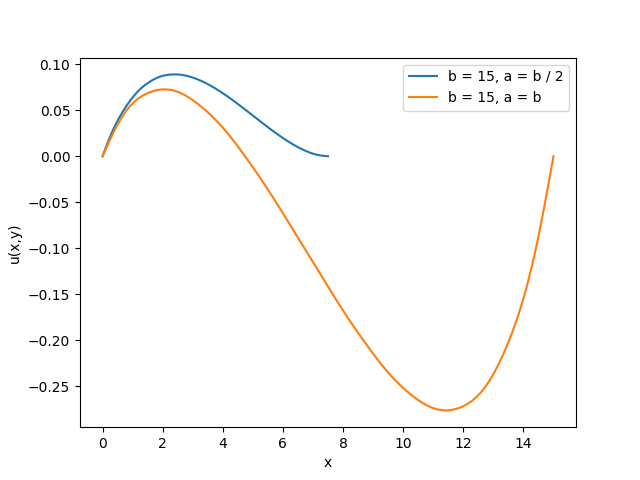
\includegraphics[width=0.49\textwidth, scale=1]{images/results/static_1/u(x,b)1.png}
        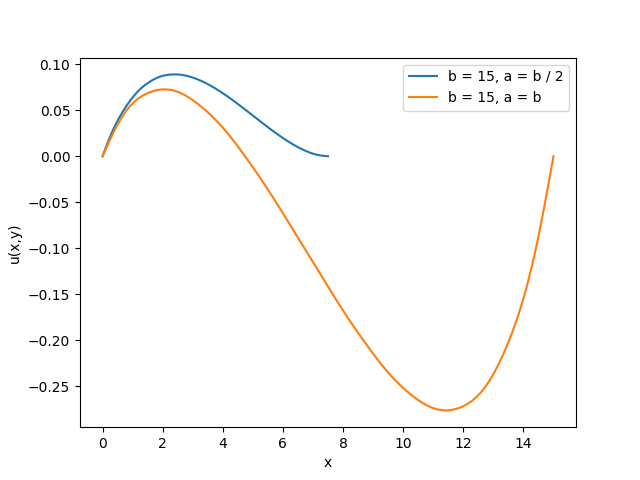
\includegraphics[width=0.49\textwidth, scale=1]{images/results/static_1/u(x,b)2.png}
        \caption{Переміщення $u(x, b)$}\label{static_1_u(x,b)}
    \end{center}
\end{figure}

На Рис. \ref{static_1_u(x,b)} зображено функція переміщеня $u(x, y)$ при $y=b$.
З графіків видно виконання граничних умов на бічних гранях $u(x,y) |_{x=0} = 0$, $u(x,y) |_{x=a} = 0$,
що підтверджує коректність знайденого розв'язку.
Також можна побачити, що при різних розмірах прямокутної області міняється максимальне та мінальне значення функції пермешінення,
при $a = 2b$ мінімум функції набуває найменьшого значення, а для випадку $a = b / 2$ максимум функції набуває найбільшого значення.

\begin{figure}[h!]
    \begin{center}
        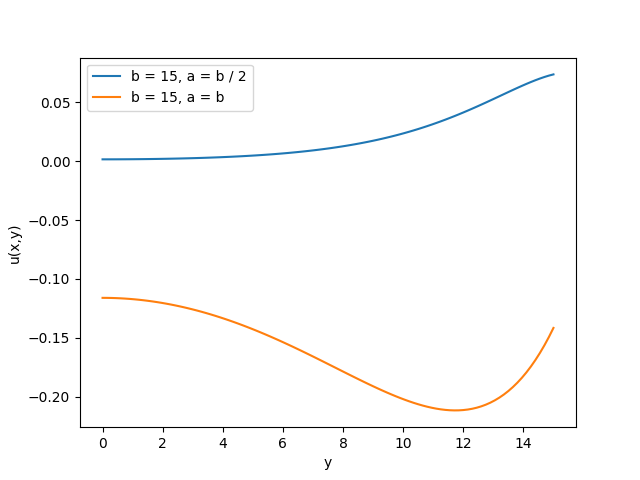
\includegraphics[width=0.49\textwidth, scale=1]{images/results/static_1/u(a:2,y)1.png}
        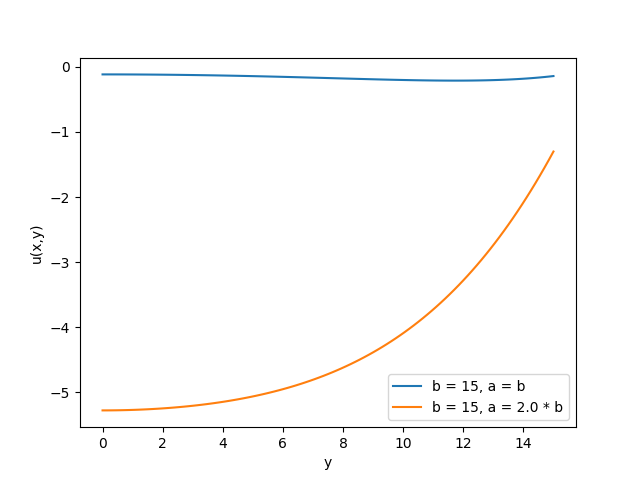
\includegraphics[width=0.49\textwidth, scale=1]{images/results/static_1/u(a:2,y)2.png}
        \caption{Переміщення $u(a/2, y)$}\label{static_1_u(a:2,y)}
    \end{center}
\end{figure}
\begin{figure}[h!]
    \begin{center}
        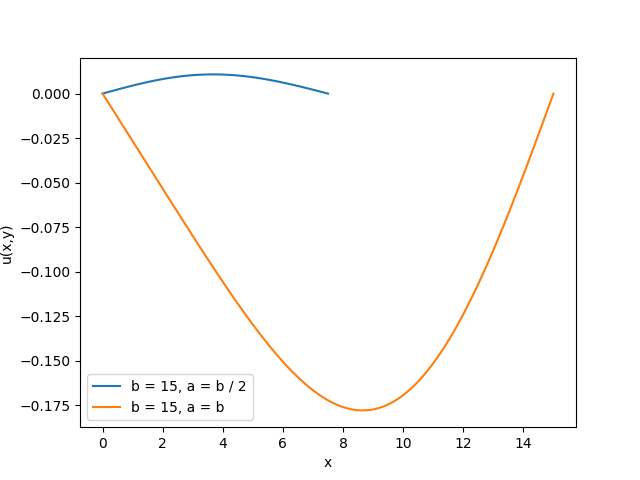
\includegraphics[width=0.49\textwidth, scale=1]{images/results/static_1/u(x,b:2)1.png}
        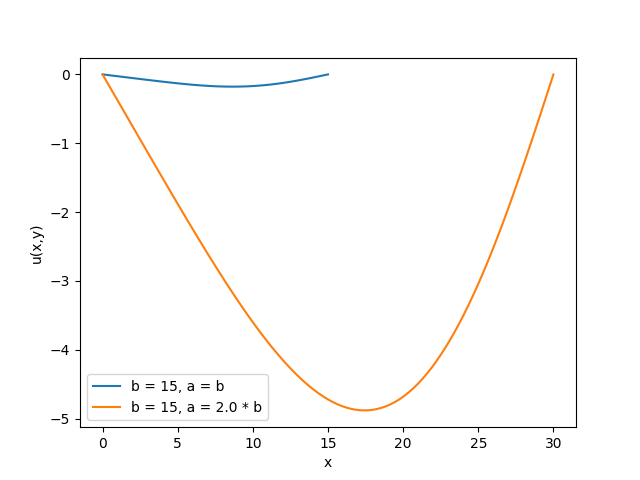
\includegraphics[width=0.49\textwidth, scale=1]{images/results/static_1/u(x,b:2)2.png}
        \caption{Переміщення $u(x, b:2)$}\label{static_1_u(x,b:2)}
    \end{center}
\end{figure}

З графіків Рис. \ref{static_1_u(a:2,y)}, Рис. \ref{static_1_u(x,b:2)} також видно,
що при збільшенні розмірів прямокутної області збільшується абсолютне значення функції переміщення.

\newpage
\begin{figure}[h!]
    \begin{center}
        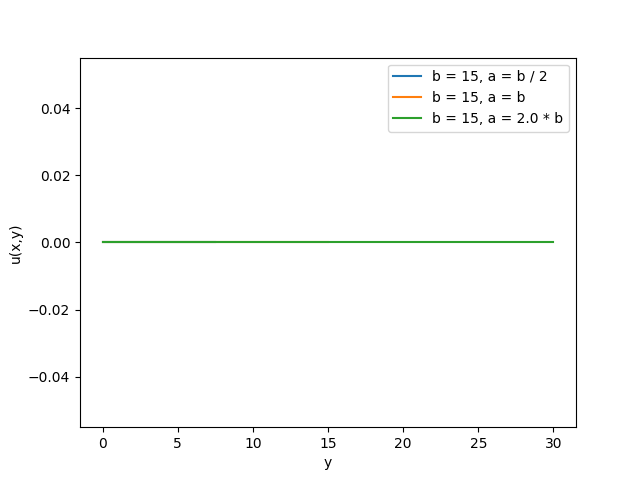
\includegraphics[width=1\textwidth, scale=0.8]{images/results/static_1/u(a,y).png}
        \caption{Переміщення $u(a, y)$}\label{static_1_u(a,y)}
    \end{center}
\end{figure}

Рис. \ref{static_1_u(a,y)} повністю підтверджує виконання граничної умови
\newline $u(x,y) |_{x=a}=0$.
Зауважимо, що на цьому графіку присутні всі три значення функції перемеіщення, які повністю накладаються одні на одну.

\begin{figure}[h!]
    \begin{center}
        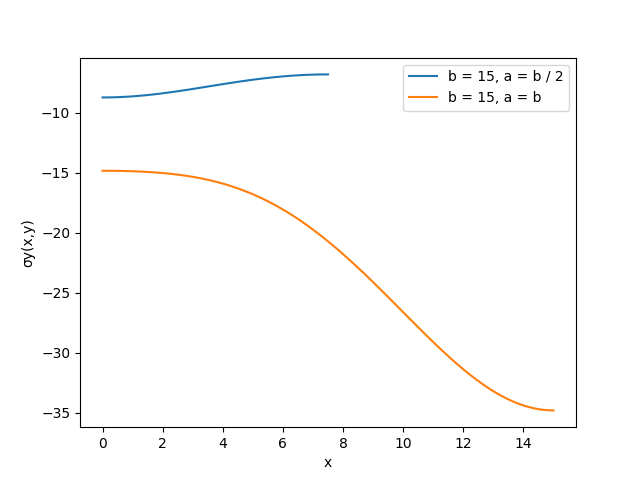
\includegraphics[width=0.49\textwidth, scale=1]{images/results/static_1/sigma_y(x,b:2)1.png}
        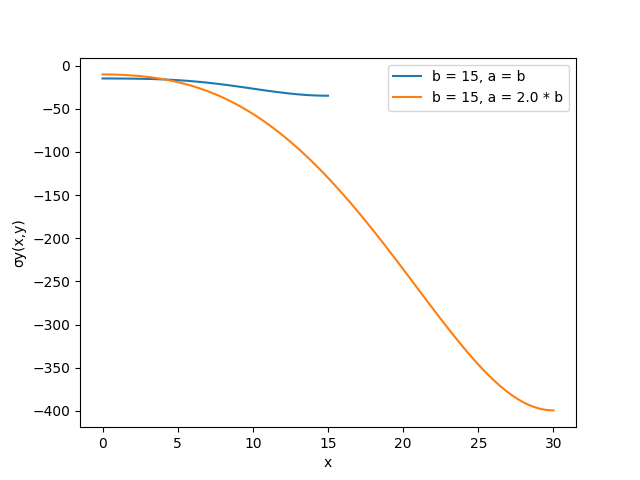
\includegraphics[width=0.49\textwidth, scale=1]{images/results/static_1/sigma_y(x,b:2)2.png}
        \caption{Напруження $\sigma_y(x, \frac{b}{2})$}\label{static_1_sigma_y(x,b:2)}
    \end{center}
\end{figure}

\begin{figure}[h!]
    \begin{center}
        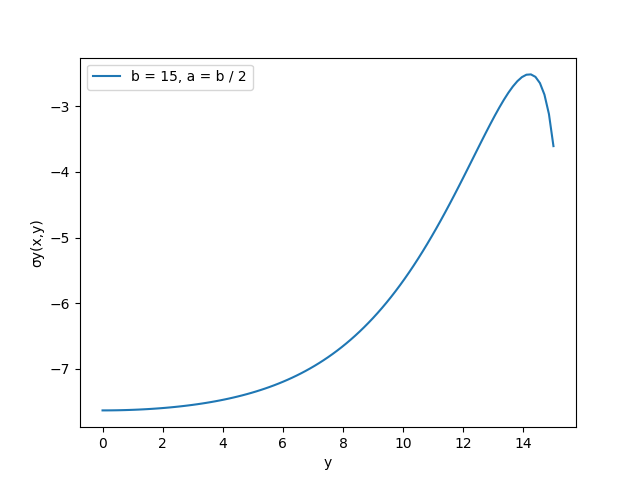
\includegraphics[width=0.49\textwidth, scale=1]{images/results/static_1/sigma_y(a,y)1.png}
        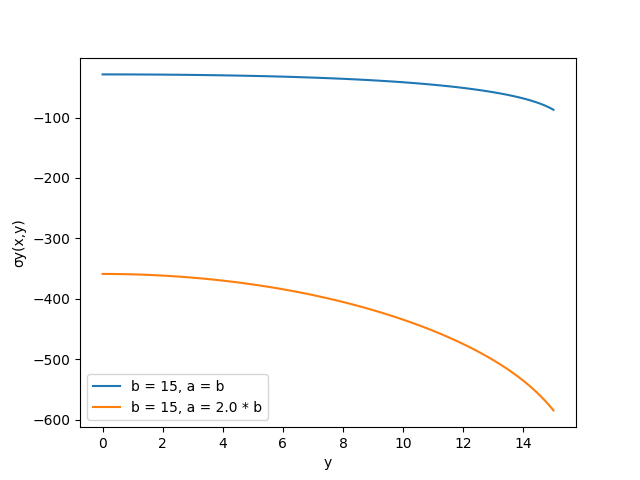
\includegraphics[width=0.49\textwidth, scale=1]{images/results/static_1/sigma_y(a,y)2.png}
        \caption{Напруження $\sigma_y(a, y)$}\label{static_1_sigma_y(a,y)}
    \end{center}
\end{figure}

\begin{figure}[h!]
    \begin{center}
        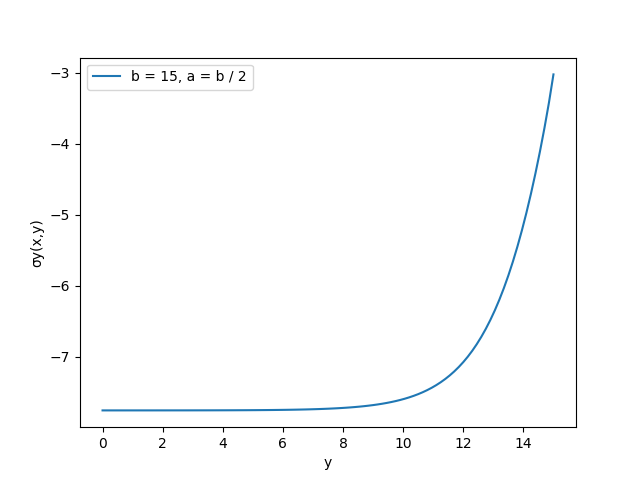
\includegraphics[width=0.49\textwidth, scale=1]{images/results/static_1/sigma_y(a:2,y)1.png}
        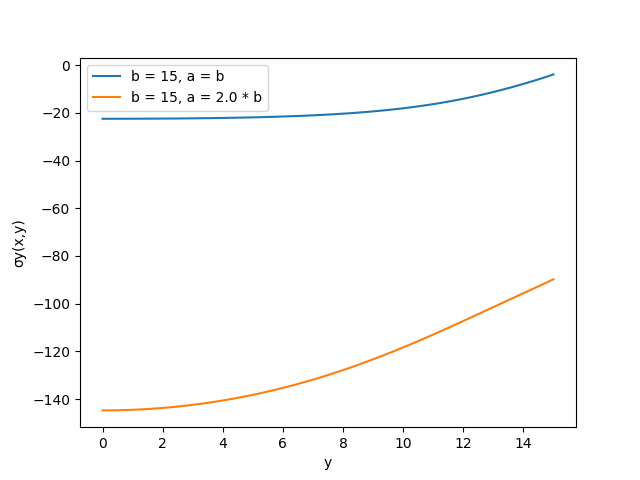
\includegraphics[width=0.49\textwidth, scale=1]{images/results/static_1/sigma_y(a:2,y)2.png}
        \caption{Напруження $\sigma_y(\frac{a}{2}, y)$}\label{static_1_sigma_y(a:2,y)}
    \end{center}
\end{figure}


\begin{figure}[h!]
    \begin{center}
        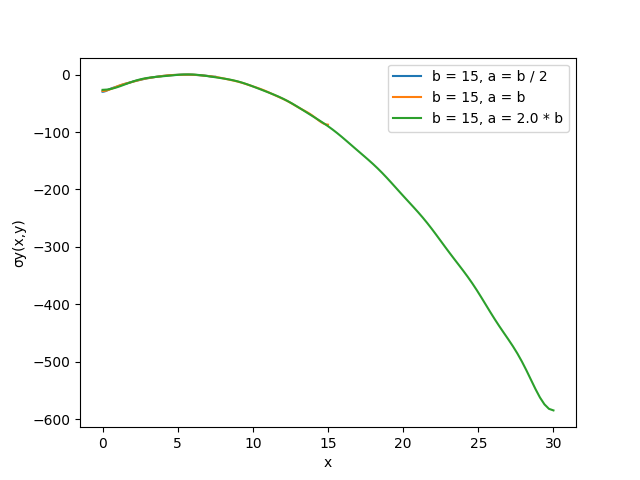
\includegraphics[width=1\textwidth, scale=1]{images/results/static_1/sigma_y(x,b).png}
        \caption{Напруження $\sigma_y(x, b)$}\label{static_1_sigma_y(x,b)}
    \end{center}
\end{figure}

З графіків Рис. \ref{static_1_sigma_y(x,b:2)} - \ref{static_1_sigma_y(x,b)} можна побачити,
що функція напруження $\sigma_y(x, y)$ в середині прямокутника (при $x=\frac{a}{2}$ або $y=\frac{b}{2}$)
міняє характер монотонності в залежності від розмірів геометричної області, а на гранях області (при $x=a$ або $y=b$)
характер залишається не змінним, лише міняються абсолютні значення функції напружень.

Також на Рис. \ref{static_1_sigma_y(x,b)} видно, що функція напруження $\sigma_y(x,y)$ повністю задовольняє граничній умові при будь-яких розмірах області
та дорівнює значенню заданного навантаженню $p(x) = (x - 5.5)^2$ на грані $y=b$.
Зауважимо, що на цьому графіку також присутні всі три значення функції перемеіщення,
які повністю накладаються одні на одну,
як і в попередньому випадку.

\begin{figure}[h!]
    \begin{center}
        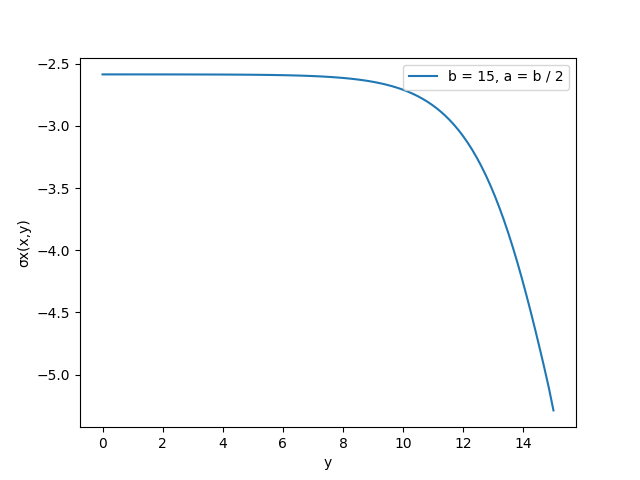
\includegraphics[width=0.49\textwidth, scale=1]{images/results/static_1/sigma_x(a:2,y)1.png}
        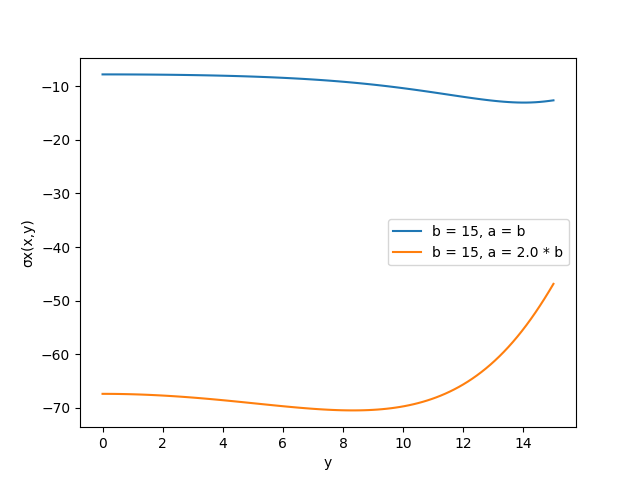
\includegraphics[width=0.49\textwidth, scale=1]{images/results/static_1/sigma_x(a:2,y)2.png}
        \caption{Напруження $\sigma_x(\frac{a}{2}, y)$}\label{static_1_sigma_x(a:2,y)}
    \end{center}
\end{figure}

\begin{figure}[h!]
    \begin{center}
        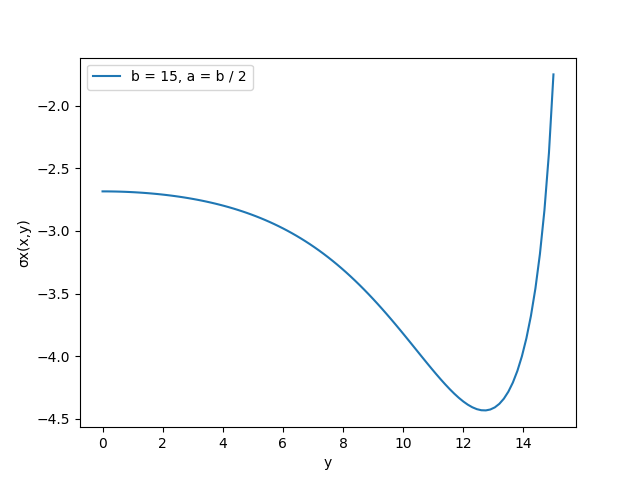
\includegraphics[width=0.49\textwidth, scale=1]{images/results/static_1/sigma_x(a,y)1.png}
        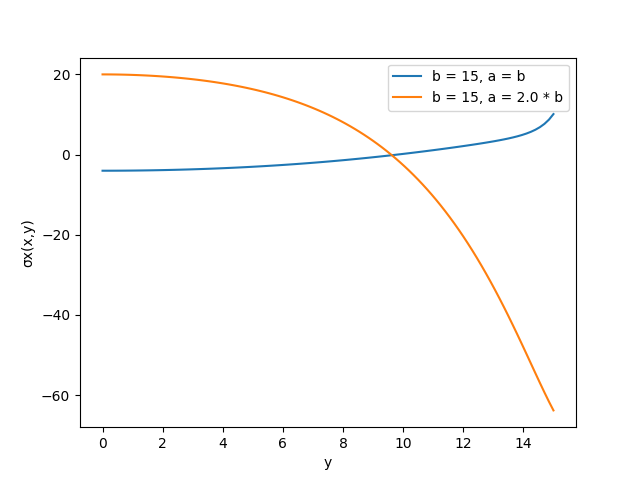
\includegraphics[width=0.49\textwidth, scale=1]{images/results/static_1/sigma_x(a,y)2.png}
        \caption{Напруження $\sigma_x(a, y)$}\label{static_1_sigma_x(a,y)}
    \end{center}
\end{figure}

Для функцій напруження $\sigma_x(x, y)$ Рис. \ref{static_1_sigma_x(a:2,y)} - \ref{static_1_sigma_x(a,y)},
аналогічно як і для попередніх функій,
при збільшенні розмірів прямокутника збільшуються абсолютні значення функції переміщення,
характер монотонності змінюється в обох випадаках: в середині області ($x=a$), та на її границі ($x=\frac{a}{2}$).


На Рис. \ref{static_1_sigma_x(x,b:2)} - \ref{static_1_sigma_x(x,b)} видно, що при зміні геометричних розмірів прямокутної області,
змінюються лише абсолютні значення функції $\sigma_x(x, y)$, її характер при фіксованих значеннях $y$ не змінюється.

\begin{figure}[h!]
    \begin{center}
        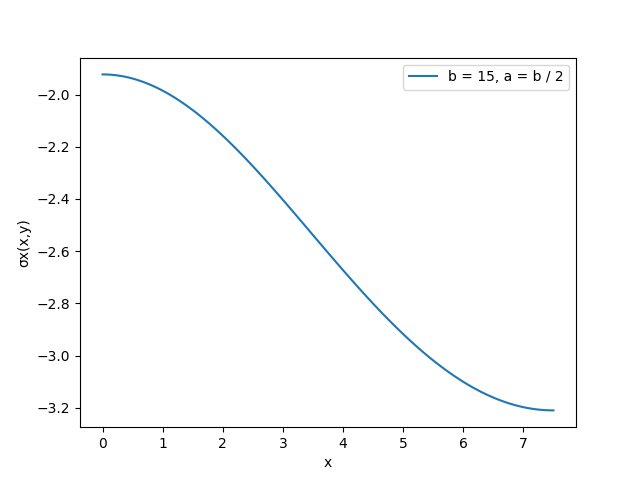
\includegraphics[width=0.49\textwidth, scale=1]{images/results/static_1/sigma_x(x,b:2)1.png}
        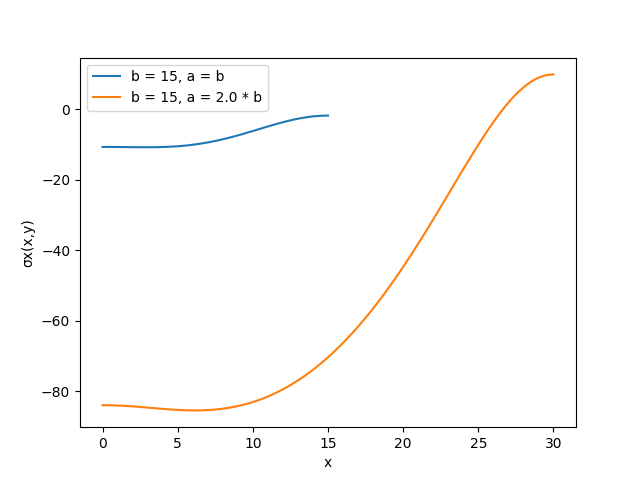
\includegraphics[width=0.49\textwidth, scale=1]{images/results/static_1/sigma_x(x,b:2)2.png}
        \caption{Напруження $\sigma_x(x, \frac{b}{2})$}\label{static_1_sigma_x(x,b:2)}
    \end{center}
\end{figure}

\begin{figure}[h!]
    \begin{center}
        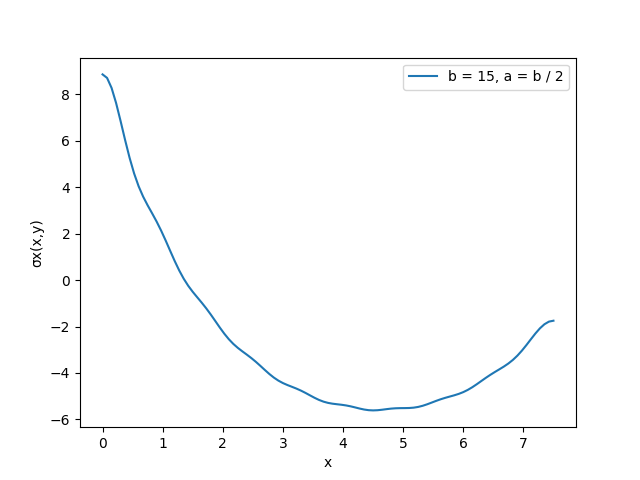
\includegraphics[width=0.49\textwidth, scale=1]{images/results/static_1/sigma_x(x,b)1.png}
        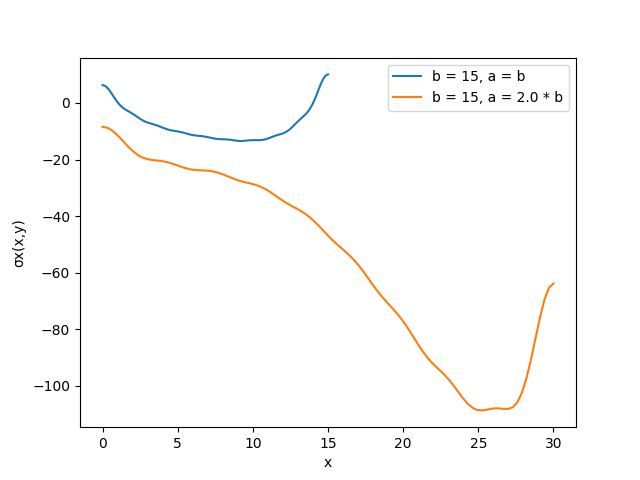
\includegraphics[width=0.49\textwidth, scale=1]{images/results/static_1/sigma_x(x,b)2.png}
        \caption{Напруження $\sigma_x(x, b)$}\label{static_1_sigma_x(x,b)}
    \end{center}
\end{figure}


% \subsubsection{Випадок граничних умов другої основної задачі теорії пружності на бічних гранях}



% \subsection{Динамічні задачі}